%!TEX root=../document.tex
\selectlanguage{ngerman}

\section{Ergebnisse}
    Die Abgabe befindet sich auf \textit{github} unter folgendem Link: \\ --> https://github.com/zcolakovic-tgm/SYT/tree/master/GK9.3
    
    \subsection{Maven}
        \textit{Maven} ist ein Buildtool und basiert auf POM - \textit{ProjekctObject Model}.
        
        \subsubsection{POM}
            Die pom.xml in einem Maven Projekt beinhaltet alle Informationen die Maven benötigt um das Projekt zu builden. Wenn man einen Task (Goal) mittels Maven ausführt, schaut diese in der pom.xml nach allen nötigen Informationen die es benötigt um das Ziel zu erreichten, und führt dann das Goal aus. Typische Dinge die festgelegt werden: 
            \begin{itemize}
                \item Project Dependencies 
                \item Plugins 
                \item Goals 
                \item Build Profiles 
            \end{itemize}
            
        \subsubsection{Features}
            Die wohl wichtigsten Features von Maven sind folgende:
            \begin{itemize}
                \item Simple project setup
                \item Dependency management
                \item Release Management (z.B. git)
            \end{itemize}
            
    \subsection{Spring}
        Hibernate wird sehr oft in Verindung mit Spring verwendet, Spring kümmert sich um die Kernfunktion einer Rest-Applikation, und zwar dem Controller. Mit Spring können auf bestimmte Links oder Link-patterns Funktionen gemapped werden, welche wiederum beispielsweise eine .jsp page aufrufen.
        
        \subsubsection{Funktionsweise}
            In Spring werden statt echten Instantiierungen so gennante Beans verwendet. Wenn ein Bean erstelltwird,handelt es sich eigentlich nur um ein Vorgehen um Instanzen der zu erstellen Spring übernimmt dabei die Aufgaben der Instantiierung, Initialisierung und des injecten an den richtigen Stellen zur Laufzeit.
            
    \subsection{Beans}
        Eine Bean ist lediglich ein Standard, welcher 3 folgende Eigenschaften vorschreibt:
        \begin{itemize}
            \item Alle Attribute sind private (nur Getter/Setter)
            \item Ein public Konstruktor ohne Parameter
            \item Muss Serializable implementieren
            \subitem  - Serializable: Beschreibt die Eigenschaft dass das Objekt in ein String umgewandelt werden kann
        \end{itemize}
    
    \subsection{Annotationen}
        \begin{itemize}
            \item \textbf{@RequestMapping}
            \subitem Ist die eigentliche Verknüpfung von Methoden und URLs. Hier wird auch festgelegt ob HTTP GET oder POST verwendet werden soll.
            
            \item \textbf{@Autowired}
            \subitem Heißt, dass Spring für die Erstellung zuständig ist. - Ermöglicht das skippen von Konfiguration welche wo anders inizialisiert wird. Bei dieser Annotation findet eine Spring initialisierung statt.
            
            \item \textbf{@Service}
            \subitem WennUserDetailsServiceImpgestartetwird,wirddasAttributuserRepositoryvomTypUserRepository definiert, und mit der @Autowired Annotation versehen. Dies bedeutet, dass nach der Bean UserRepository gesucht wird, und diese dann anschließend in dieses Attribut ”injected” wird. Ich habe noch immer nicht ganz verstanden was ”injecten” bedeutet in dem Kontext.
            
            \item \textbf{@Configuration}
	        \subitem Verweißt darauf, dass in der Klasse eine oder mehrere Beans vorhanden ist. 
	        
            \item\textbf{@EnableWebSecurity}
	        \subitem Rolle eines Makers. Es erlaubt Spring zu finden und wendet es automatisch auf den globalen WebSecurity. 
	        
	        \item \textbf{@Entity} 
	        \subitem Eine DB-Tabelle wird hiermit definiert 
	        
	        \item \textbf{@Table} 
	        \subitem Bestimmt den namen der Tabelle in der DB (default ist Name der Klasse) 
	        
	        \item \textbf{@Id} 
	        \subitem Dient zur festlegung des PK (Primary Key)
            
            \item \textbf{@GeneratedValue} 
            \subitemagt JPA, dass sie sich selbst um die festlegung der ID kümmern muss 
            
            \item \textbf{@Transient} 
            \subitem Dient um ein Feld als nicht persistent zu setzten (Runtime-Use) 
            
            \item \textbf{@ManyToMany} 
            \subitem Viele- zu viele Beziehung zwischen zwei Entitäten @JoinTable @JoinColumn definiert das die Attribute welche die Fremdschlüssel beinhalten 
            
            \item \textbf{@mappedBy}
            \subitem Ist das Gegenteil von @JoinColumn

        \end{itemize}
    
    \subsection{Implementation und Aufbau}
        Folgendes Beispiel wurde als Basis genutzt: \textit{https://hellokoding.com/registration-and-login-example-with-spring-security-spring-boot-spring-data-jpa-hsql-jsp/}
        
        \newpage
       
        \subsubsection{Projektstruktur}
            
            \begin{figure}[h]
        	    \centering
        		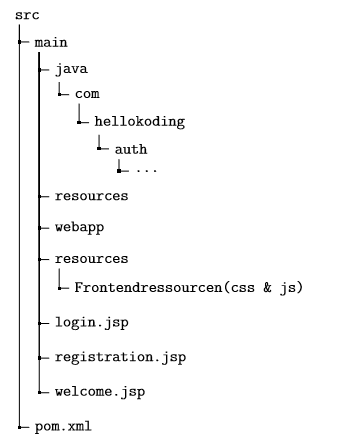
\includegraphics[width=0.5\textwidth]{images/Unbenannt.PNG}
        	    \caption{Aufbau - Projektstruktur}
            \end{figure}
        
        \newpage
        
            \begin{figure}[h]
        	    \centering
        		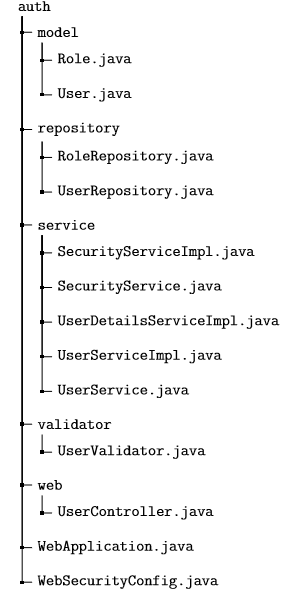
\includegraphics[width=0.5\textwidth]{images/Unbenannt2.PNG}
        	    \caption{Aufbau - Klassenstruktur}
            \end{figure}
            
        \clearpage
        \subsubsection{Lauffähigkeit}
             Das Projekt wurde zuerst aus dem Repository geclont. Darauf hin mittels \textit{-> File -> Import -> Exisiting Maven Projekt}, in Eclipse (Oxygen) importieren.
        
            In der Running Config (\textit{RunAS -> maven build} als Goal \textit{spring-boot:run} setzen.
            
        \subsubsection{Dependencies}
        Die Abhängigkeiten für das Projekt (Maven beschrieben) sind in der pom.xml (Project Object Model) eingespeichert.
            \begin{lstlisting}[language = java]
                <?xml version="1.0" encoding="UTF-8"?>
                <project xmlns="http://maven.apache.org/POM/4.0.0" xmlns:xsi="http://www.w3.org/2001/XMLSchema-instance" xsi:schemaLocation="http://maven.apache.org/POM/4.0.0 http://maven.apache.org/xsd/maven-4.0.0.xsd">
                    <modelVersion>4.0.0</modelVersion>
                    <artifactId>auth</artifactId>
                    <name>auth</name>
                    <description>auth</description>
                    <packaging>war</packaging>
                    <parent>
                        <groupId>org.springframework.boot</groupId>
                        <artifactId>spring-boot-starter-parent</artifactId>
                        <version>1.3.5.RELEASE</version>
                    </parent>
                
                    <properties>
                        <project.build.sourceEncoding>UTF-8</project.build.sourceEncoding>
                        <java.version>1.7</java.version>
                    </properties>
                
                    <dependencies>
                        <dependency>
                            <groupId>org.springframework.boot</groupId>
                            <artifactId>spring-boot-starter-web</artifactId>
                        </dependency>
                
                        <dependency>
                            <groupId>org.springframework.boot</groupId>
                            <artifactId>spring-boot-starter-data-jpa</artifactId>
                        </dependency>
                
                        <dependency>
                            <groupId>org.springframework.boot</groupId>
                            <artifactId>spring-boot-starter-security</artifactId>
                        </dependency>
                
                        <dependency>
                            <groupId>org.hsqldb</groupId>
                            <artifactId>hsqldb</artifactId>
                            <scope>runtime</scope>
                        </dependency>
                
                        <dependency>
                            <groupId>org.springframework.boot</groupId>
                            <artifactId>spring-boot-starter-tomcat</artifactId>
                            <scope>provided</scope>
                        </dependency>
                
                        <dependency>
                            <groupId>org.apache.tomcat.embed</groupId>
                            <artifactId>tomcat-embed-jasper</artifactId>
                            <scope>provided</scope>
                        </dependency>
                
                        <dependency>
                            <groupId>javax.servlet</groupId>
                            <artifactId>jstl</artifactId>
                        </dependency>
                    </dependencies>
                    <build>
                        <plugins>
                            <plugin>
                                <groupId>org.springframework.boot</groupId>
                                <artifactId>spring-boot-maven-plugin</artifactId>
                            </plugin>
                        </plugins>
                    </build>
                </project>    
            \end{lstlisting}
            \captionof{lstlisting}{pom.xml}
            
        \subsubsection{Model}
            Im Model befinden sich 2 JPA-Einträge (Java Persistence API) für dieses Projekt. In diesen Klassen werden Elemente definiert die in der Datenbank gespeichert werden sollen. Dies passiert mittels object-relational mapping. Was soviel bedeutet, wie das eine Datenbank wie normale Javaobjekte verwendet werden können (POJO). Es können auch hier schon Methoden wie Setter und Getter definiert werden, welche oft gebraucht. Bei dieser Klasse handelt es sich um die Definition für Benutzer des Projektes. Annotations (@) dienen zur definition von Eigenschaften. 
            \begin{lstlisting}[language = java]
                @Entity
                @Table(name = "user")
                public class User {
                    private Long id;
                    private String username;
                    private String password;
                    private String passwordConfirm;
                    private Set<Role> roles;
                
                    @Id
                    @GeneratedValue(strategy = GenerationType.AUTO)
                    public Long getId() {
                        return id;
                    }
                
                    public void setId(Long id) {
                        this.id = id;
                    }
                
                    public String getUsername() {
                        return username;
                    }
                
                    public void setUsername(String username) {
                        this.username = username;
                    }
                
                    public String getPassword() {
                        return password;
                    }
                
                    public void setPassword(String password) {
                        this.password = password;
                    }
                
                    @Transient
                    public String getPasswordConfirm() {
                        return passwordConfirm;
                    }
                
                    public void setPasswordConfirm(String passwordConfirm) {
                        this.passwordConfirm = passwordConfirm;
                    }
                
                    @ManyToMany
                    @JoinTable(name = "user_role", joinColumns = @JoinColumn(name = "user_id"), inverseJoinColumns = @JoinColumn(name = "role_id"))
                    public Set<Role> getRoles() {
                        return roles;
                    }
                
                    public void setRoles(Set<Role> roles) {
                        this.roles = roles;
                    }
                }
            \end{lstlisting}
            \captionof{lstlisting}{User JPA Klasse}
        
        \subsubsection{Repository}
            Spring Data JPA besitzt eingebaute Funktionalitäten. in Repository werden einige davon implementiert um Datenbankaufgaben zu übernehmen (zB findOne, findAll, save) 
            
            \begin{lstlisting}[language = java]
                public interface UserRepository extends JpaRepository<User, Long> { 
                    User findByUsername(String username); 
                }
            \end{lstlisting}
            \captionof{lstlisting}{User Repository Klasse}
            
            Im folgendem Beispiel wird ein findByUsername aktiviert:
            
            \begin{lstlisting}[language = java]
                @Service 
                public class UserDetailsServiceImpl implements UserDetailsService{ 
                    @Autowired 
                    private UserRepository userRepository;
    
                    @Override 
                    @Transactional(readOnly = true) 
                    public UserDetails loadUserByUsername(String username) throws UsernameNotFoundException { 
                        User user = userRepository.findByUsername(username);
                        Set<GrantedAuthority> grantedAuthorities = new HashSet<>(); 
                        for (Role role : user.getRoles()){ 
                            grantedAuthorities.add(new SimpleGrantedAuthority(role.getName()));
                        }
                        return new org.springframework.security.core.userdetails.User(user.getUsername() , user. getPassword() , grantedAuthorities);
                    }
                }
            \end{lstlisting}
            \captionof{lstlisting}{UserDataService} 
            
            UserDetailsServiceImpl.java dient als Klasse welche einem anhand des Usernames den gesamten Nutzer mit seinen Daten zurück gibt. \\
            
            SecurityService.java wird verwendet um den aktuell angemeldeten Benutzer die Accounts zu übergeben & User die sich gerade angelegt haben automatisch einzuloggen. \\
                
            UserServiceImpl.java dient für die Erstellung von Benutzern. Dabei wird der anzulegende Benutzer als Parameter mitgegeben, aus diesem werden dann alle Attribute ausgelesen und zur DB hinzugefügt. \\
            
            \newpage 
            
            \begin{lstlisting}[language = java]
                @Override 
                public void save(User user) {     
                    user.setPassword(bCryptPasswordEncoder.encode(user.getPasswod(); 
                    user.setRoles(new HashSet<>(roleRepository.findAll())); 
                    userRepository.save(user); 
                }  
            \end{lstlisting}
            \captionof{lstlisting}{Benutzer Erstellung}
            
        \subsubsection{Validator}
            Dient zur Überprüfung der Gültigkeit der Daten die der Benutzer angibt beim Erstellen seines Accountes.
            
            \begin{lstlisting}[language = java]
                @Component
                public class UserValidator implements Validator {
                    @Autowired
                    private UserService userService;
                
                    @Override
                    public boolean supports(Class<?> aClass) {
                        return User.class.equals(aClass);
                    }
                
                    @Override
                    public void validate(Object o, Errors errors) {
                        User user = (User) o;
                
                        ValidationUtils.rejectIfEmptyOrWhitespace(errors, "username", "NotEmpty");
                        if (user.getUsername().length() < 6 || user.getUsername().length() > 32) {
                            errors.rejectValue("username", "Size.userForm.username");
                        }
                        if (userService.findByUsername(user.getUsername()) != null) {
                            errors.rejectValue("username", "Duplicate.userForm.username");
                        }
                
                        ValidationUtils.rejectIfEmptyOrWhitespace(errors, "password", "NotEmpty");
                        if (user.getPassword().length() < 8 || user.getPassword().length() > 32) {
                            errors.rejectValue("password", "Size.userForm.password");
                        }
                
                        if (!user.getPasswordConfirm().equals(user.getPassword())) {
                            errors.rejectValue("passwordConfirm", "Diff.userForm.passwordConfirm");
                        }
                    }
                }
            \end{lstlisting}
            \captionof{lstlisting}{UserValidator}
            
            Es werden die klassischen Überprüfungen wie Länge des Benutzernamens oder des Passwort vorgenommen. Es kontrolliert außerdem ob die Felder überhaupt befüllt wurden. Fehlermeldungen wurden in validation.properties festgelegt.
        
        \newpage
        
        \subsubsection{Web}
            Die Aufgabe des UserController ist es die Methoden mit URLs zu verknüpfen. So benötigt es eine bestimmte URL um eine bestimmte Methode aufzurufen.
            
            \begin{lstlisting}[language = java]
                @Controller
                public class UserController {
                    @Autowired
                    private UserService userService;
                
                    @Autowired
                    private SecurityService securityService;
                
                    @Autowired
                    private UserValidator userValidator;
                
                    @RequestMapping(value = "/registration", method = RequestMethod.GET)
                    public String registration(Model model) {
                        model.addAttribute("userForm", new User());
                
                        return "registration";
                    }
                
                    @RequestMapping(value = "/registration", method = RequestMethod.POST)
                    public String registration(@ModelAttribute("userForm") User userForm, BindingResult bindingResult, Model model) {
                        userValidator.validate(userForm, bindingResult);
                
                        if (bindingResult.hasErrors()) {
                            return "registration";
                        }
                
                        userService.save(userForm);
                
                        securityService.autologin(userForm.getUsername(), userForm.getPasswordConfirm());
                
                        return "redirect:/welcome";
                    }
                
                    @RequestMapping(value = "/login", method = RequestMethod.GET)
                    public String login(Model model, String error, String logout) {
                        if (error != null)
                            model.addAttribute("error", "Your username and password is invalid.");
                
                        if (logout != null)
                            model.addAttribute("message", "You have been logged out successfully.");
                
                        return "login";
                    }
                
                    @RequestMapping(value = {"/", "/welcome"}, method = RequestMethod.GET)
                    public String welcome(Model model) {
                        return "welcome";
                    }
                }
            \end{lstlisting}
            \captionof{lstlisting}{UserController}